\documentclass[a4paper]{article}
\usepackage[utf8]{inputenc}
\usepackage{amsmath}
\usepackage{siunitx}
\usepackage[ngerman]{babel}
\usepackage{pgfplots}
\usepackage{hyperref}
\usepackage{pgfplotstable}
\usepackage[section]{placeins}
\usepackage{enumitem}
\usepackage{float}
\usepackage{booktabs}
\usepackage[normalem]{ulem}
\usepackage{subcaption}
\usepackage{chngpage}

\pgfplotsset{compat=1.15}

% Full Reference, produces: "Abbildung 3: Schaltplan"
\newcommand*{\fullref}[1]{\hyperref[{#1}]{\autoref*{#1}: \nameref*{#1}}}

\title{GPET\\ Auswertung Versuch 7\\ Gruppe 1}

\author{Jonas Otto\\ \href{mailto:jonas@jonasotto.com}{jonas@jonasotto.com} 
   \and Luca Krüger \\ \href{mailto:luca.krueger@uni-ulm.de}{luca.krueger@uni-ulm.de} }
\date{vom   29. Mai 2018}

\begin{document}
    
\maketitle
\newpage
\section{Versuchsauswertung}

\subsection{Spannungsfolger}
\begin{figure}[H]
    \centering
    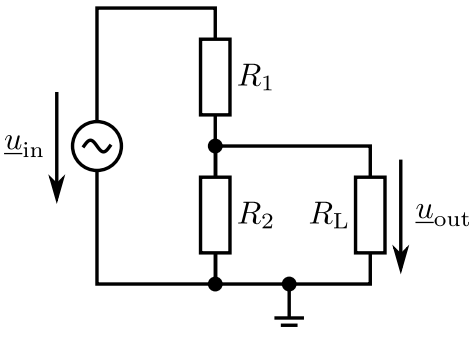
\includegraphics[width=0.8\textwidth]{versuch1/aufbau-spannungsteiler.png}
    \caption{Belasteter Spannungsteiler}
    \label{fig:versuch1-spannungsfolger-aufbau-spannungsteiler}
\end{figure}



Beim belasteten Spannungsteiler  (Abbildung \ref{fig:versuch1-spannungsfolger-aufbau-spannungsteiler}) ändert sich die zu erwartende Ausgangsspannung beim Anschließen einer Last, da der zweite Widerstand im Spannungsteiler parallel zur Last geschaltet ist. Die gemessene Ausgangsspannung beträgt $0.775\si{V}$, nicht $2.5\si{V}$. Beim belasteten Spannungsfolger (Abbildung \ref{fig:versuch1-spannungsfolger-aufbau-spannungsfolger}) hingegen hat die Last keinen Einfluss auf den Spannungsteiler, da der Spannungsteiler nur an den Eingang des OP angeschlossen ist. In den Eingang fließt aufgrund des sehr hohen Eingangswiderstand kein Strom. Die gemessene Spannung beträgt $~2.5\si{V}$, entspricht damit also dem erwartete Wert des unbelasteten Spannungsteilers. Eine solche Schaltung kann immer dort verwendet werden, wo eine Last einen unerwünschten Einfluss auf die Wirkungsweise der Schaltung hat, z.B. bei Filtern.

\begin{figure}[H]
    \centering
    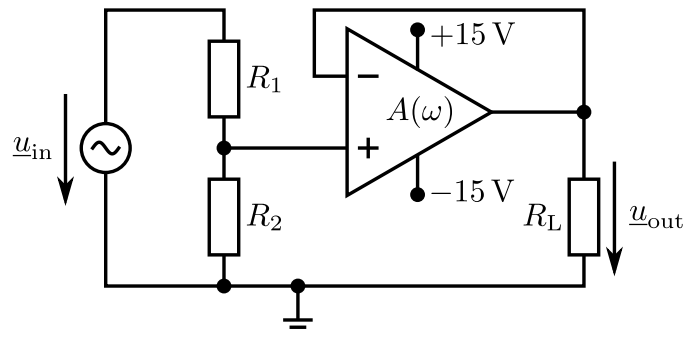
\includegraphics[width=0.8\textwidth]{versuch1/aufbau-spannungsfolger.png}
    \caption{Belasteter Spannungsfolger}
    \label{fig:versuch1-spannungsfolger-aufbau-spannungsfolger}
\end{figure}

\subsection{Charakterisierung der Verstärkung}
\label{subsec:versuch2-verstaerkung}

Im folgenden wurde ein invertierender Verstärker wie in Abbildung \ref{fig:versuch2-aufbau} aufgebaut.
Da $A_B=\frac{R_2}{R_1}$ gilt und $R_1=1\si{k\ohm}$ wird für eine Verstärkung $A_B=10$ der Widerstand $R_2=10\si{k\ohm}$ gewählt.

\begin{figure}[H]
    \centering
    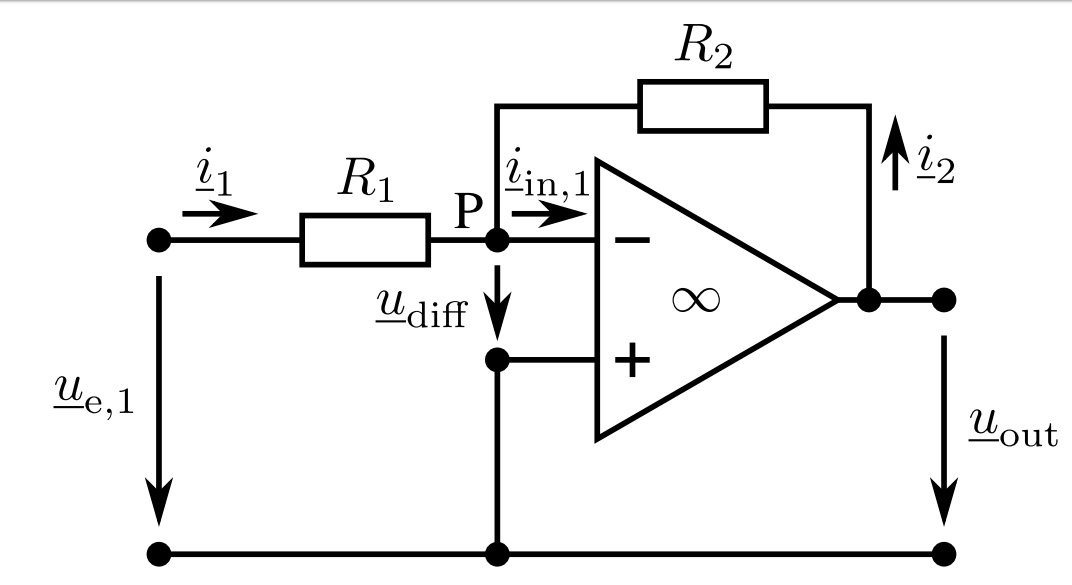
\includegraphics[width=0.8\textwidth]{versuch2/aufgabe2.png}
    \caption{Invertierender Verstärker}
    \label{fig:versuch2-aufbau}
\end{figure}

\begin{table}[H]
\begin{adjustwidth}{-2in}{-2in}
    \begin{center}
    \begin{tabular}{l *{10}{S[table-format=2.2, tight-spacing=true] }}
        \toprule
        {$\underline{u}_\text{in} [\si{Vpp}]$} & 0.5 & 1.0 & 1.5 & 2.0 & 2.5 & 3.0 & 3.5 & 4.0 & 4.5 & 5.0\\
        \midrule
        {$\underline{u}_\text{out} [\si{Vpp}]$} & 0.51 & 1.01 & 1.22 & 1.35 & 1.45 & 1.53 & 1.61 & 1.65 & 1.71 & 1.75\\
        {$A_B = \underline{u}_\text{out} / \underline{u}_\text{in}$} & 1.02 & 1.01 & 0.81 & 0.68 & 0.58 & 0.51 & 0.46 & 0.41 & 0.38 & 0.35\\
        {$20 \si{dB} \log_{10}(A_B) [\si{dB}]$} & 0.17 & 0.09 & -1.83 & -3.35 & -0.47 & -5.85 & -6.75 & -7.74 & -8.40 & -9.12\\
        \bottomrule
    \end{tabular}

    \caption{Messtabelle : Amplitudenabhängigkeit}
    \label{tab:2a-messtab-amplitude}
    \end{center}
    \end{adjustwidth}
\end{table}

\begin{figure}[H]
    \centering
    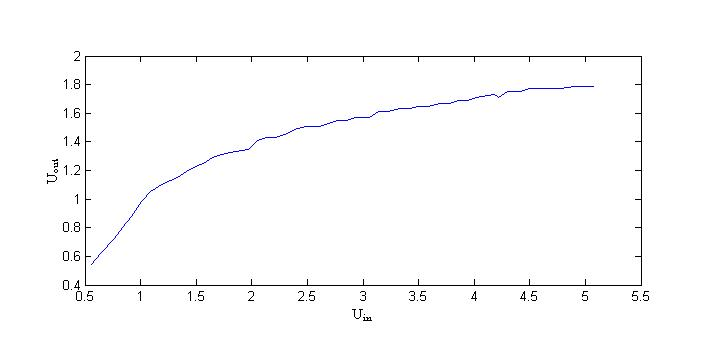
\includegraphics[width=0.8\textwidth]{versuch2/V2_Amplitude.jpg}
    \caption{Amplitudenabhängigkeit}
    \label{fig:versuch2-sweep-amplitude}
\end{figure}

Wie in Tabelle \ref{tab:2a-messtab-amplitude} und Abbildung \ref{fig:versuch2-sweep-amplitude} zu sehen, ändert sich die Verstärkung bei steigender Amplitude. Bei steigender Amplitude nimmt die Verstärkung ab. Ab ca. $3\si{V}$ steigt die Spannung kaum mehr an.

\begin{table}[H]
\begin{adjustwidth}{-2in}{-2in}  
    \begin{center}
    \begin{tabular}{l *{6}{S[table-format=2.2, tight-spacing=true] }}
        \toprule
        {$f [\si{Hz}]$} & {$10^1$} & {$10^2$} & {$10^3$} & {$10^4$} & {$10^5$} & {$10^6$}\\
        {$\underline{u}_\text{in} [\si{Vpp}]$} & 2 & 2 & 2 & 2 & 2 & 2\\
        \midrule
        {$\underline{u}_\text{out} [\si{Vpp}]$} & 1.77 & 1.77 & 1.67 & 1.39 & 1.32 & 0.46 \\
        {$A_B = \underline{u}_\text{out} / \underline{u}_\text{in}$} & 0.88 & 0.88 & 0.82 & 0.69 & 0.66 & 0.23\\
        {$20 \si{dB} \log_{10}(A_B) [\si{dB}]$} & -1,11 & -1.11 & -1.72 & -3.22 & -3.61 & -12.76\\
        \bottomrule
    \end{tabular}

    \caption{Messtabelle: Frequenzabhängigkeit}
    \label{tab:2a-messtab-frequenz}
    \end{center}
    \end{adjustwidth}
\end{table}

\begin{figure}[H]
    \centering
    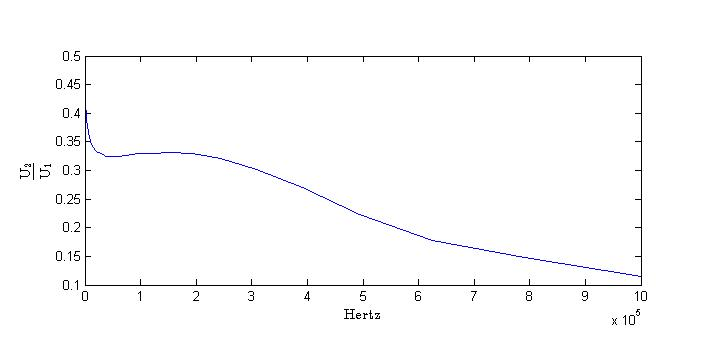
\includegraphics[width=0.8\textwidth]{versuch2/V2_Frequenz.jpg}
    \caption{Frequenzabhängigkeit}
    \label{fig:versuch2-sweep-frequenz}
\end{figure}

In Tabelle \ref{tab:2a-messtab-frequenz} und Abbildung \ref{fig:versuch2-sweep-frequenz} ist die Frequenzabhängigkeit des invertierenden Verstärkers dargestellt. Die $3\si{dB}$ Grenzfrequenz liegt bei etwas unter $10\si{kHz}$, wie aus der Messtabelle ersichtlich.
\\
\underline{Anmerkung:} Zu Beginn diesen Versuches wurde der Widerstand $R_2$ bewusst so gewählt, dass ein Übertragungsverhältnis von $A_B=10$ zustande kommt. Dies der Messtabelle zufolge nicht der Fall. Während diesem Versuch musste auf die Schaltung einer benachbarten Gruppe zurückgegriffen werden, da die eigenen Messgeräte fehlerhaft waren. Möglicherweise wurde in der Schaltung der anderen Gruppe noch nicht der Widerstand $R_2$ ersetzt, was die Unterschiede zum erwarteten Übertragungsverhältnis erklären könnte. Beim Ablesen der Messwerte ist dieser Fehler auch noch nicht aufgefallen, erst später bei der Berechnung der Verhältnisse. Die oben getroffenen Aussagen sollten allerdings auch für ein Übertragungsverhältnis von $A_B=10$ gültig sein.
\subsection{Addierer}
%Berechnet: Uout=-10.42V
%Verstärkung: 5/3 bzw 5/2

Die Verstärkung für $\underline{u}_{e,1}$ beträgt $\frac{R_{11}}{R_2}=\frac{500\si{\ohm}}{300\si{\ohm}}=\frac{5}{3}$, für $\underline{u}_{e,2}$ beträgt diese $\frac{5}{2}$. Daraus ergibt sich eine berechnete Ausgangsspannung von $u_{out}=-10.42\si{V}$.
Die Amplitude der gemessenen Ausgangsspannung (Abbildung \ref{fig:versuch3-addierer-screenshot}) beträgt $3.66\si{V}$, es gibt aber einen negativen Gleichanteil. Die verstärkte Gleichspannung wird also mit der verstärkten Wechselspannung überlagert.

\begin{figure}[H]
    \centering
    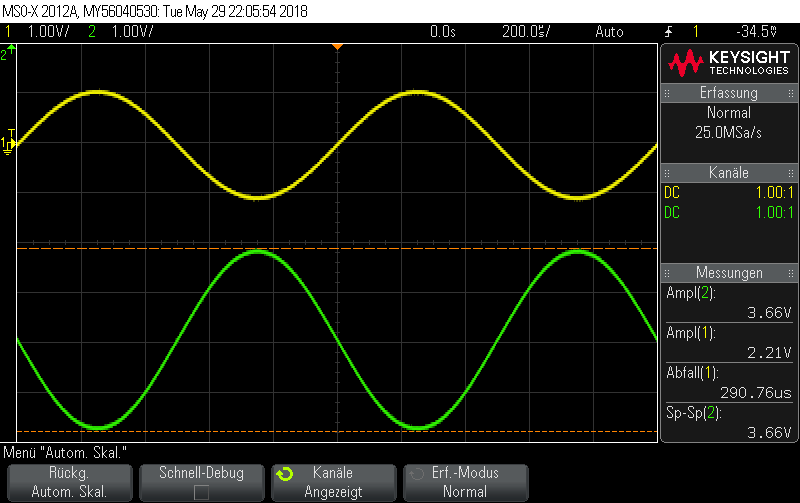
\includegraphics[width=0.8\textwidth]{versuch3/scope_18.png}
    \caption{Messung der Ausgangsspannung des Addierers}
    \label{fig:versuch3-addierer-screenshot}
\end{figure}

\subsection{Integrator}

In diesem Versuch wird ein Integrator (Abbildung \ref{fig:versuch4-aufbau-integrator}) mit folgenden Bauteilwerten aufgebaut: $R_1=R_2=1\si{k\ohm}$, $R_3=220\si{k\ohm}$ und $C=1.5\si{nF}$.
\begin{figure}[H]
    \centering
    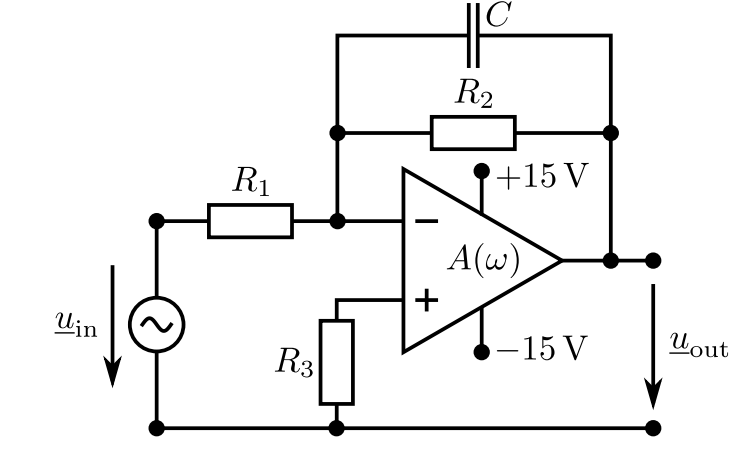
\includegraphics[width=0.8\textwidth]{versuch4/aufbau-integrator.png}
    \caption{Integratorschaltung}
    \label{fig:versuch4-aufbau-integrator}
\end{figure}

Ab einer Frequenz von $300\si{kHz}$ funktioniert die Integration. Das heißt, es wird ein Sinus/Cosinus integriert und damit entspricht die Phasenverschiebung $\ang{90}$ gegenüber dem Eingangssignal.


\begin{figure}[H]
    \centering
    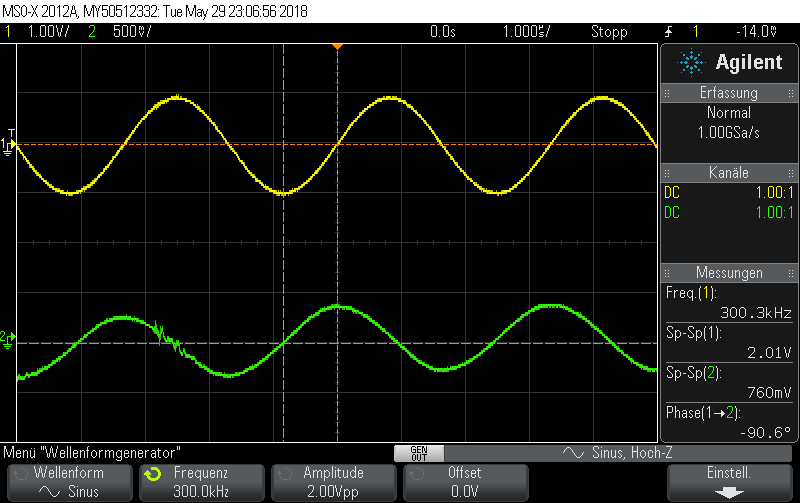
\includegraphics[width=0.8\textwidth]{versuch4/versuch4_phase.png}
    \caption{Phasenverschiebung bei Integration}
    \label{fig:versuch4-phase}
\end{figure}

Auch bei Rechteck- oder Sägezahnspannung findet eine Integration statt.
Bei der Rechteckspannung sind zudem Spitzen beim Umschalten zu erkennen. Dies liegt daran, dass der Kondensator noch geladen ist und sich erst langsamer über den Widerstand entlädt.
Bei einer Sägezahnspannung wird eine quadratische Integration erwartet. Dies bestätigt sich in der Messung, wie in (Abbildung \ref{fig:versuch4-dreieck}) ersichtlich.

\begin{figure}[H]
    \centering
    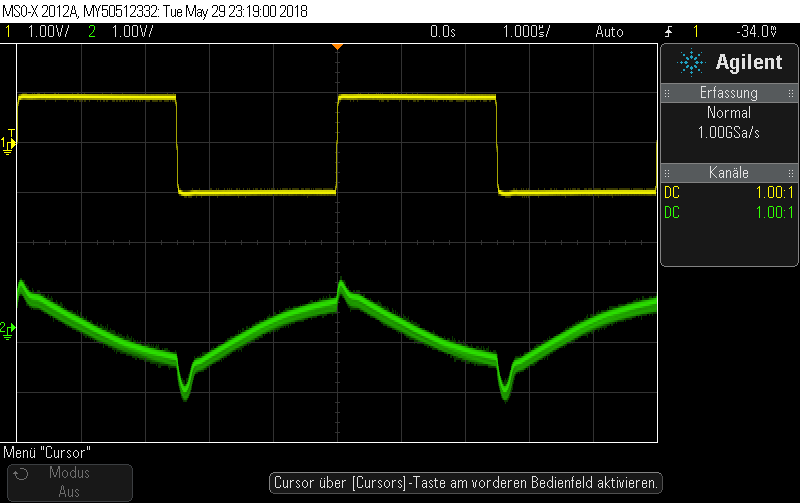
\includegraphics[width=0.8\textwidth]{versuch4/versuch4_rechteck.png}
    \caption{Integration einer Rechteckspannung}
    \label{fig:versuch4-rechteck}
\end{figure}

\begin{figure}[H]
    \centering
    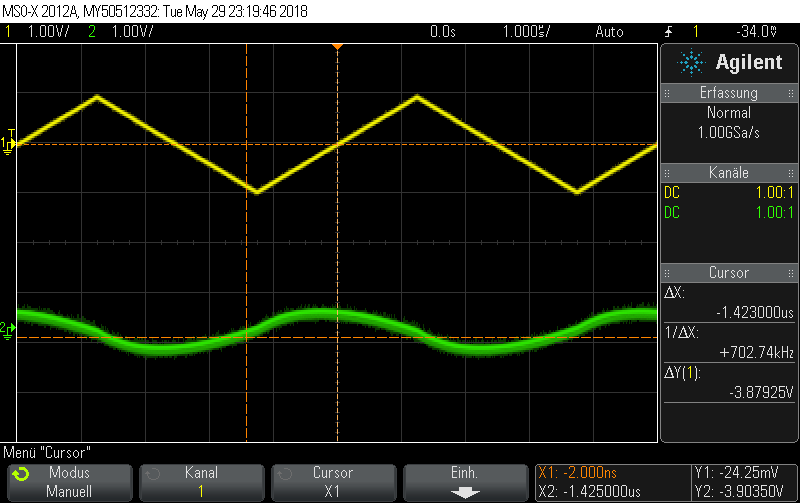
\includegraphics[width=0.8\textwidth]{versuch4/versuch4_saegezahn.png}
    \caption{Integration einer Sägezahnspannung}
    \label{fig:versuch4-dreieck}
\end{figure}

Der Frequenzgang (Abbildung \ref{fig:versuch4-sweep1}) zeigt, dass das Übertragungsverhältnis bei kleinen Frequenzen $1$ beträgt und zwischen $10\si{kHz}$ und $100\si{kHz}$ stark abfällt. Die Grenzfrequenz liegt bei ungefähr $100\si{kHz}$.

\begin{figure}[H]
    \centering
    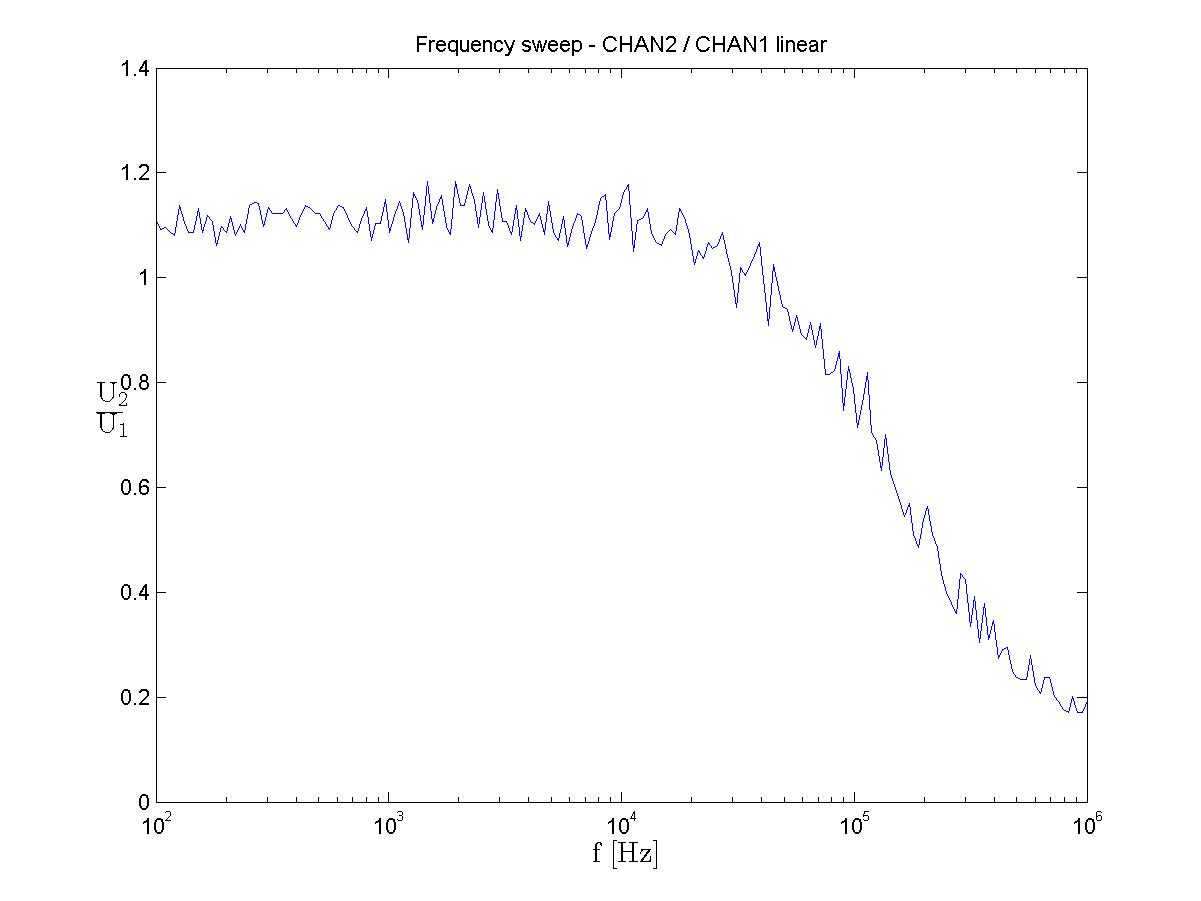
\includegraphics[width=0.8\textwidth]{versuch4/versuch4_sweep1_frequencysweep_ylinxlog.jpg}
    \caption{Frequenzgang des Integrators}
    \label{fig:versuch4-sweep1}
\end{figure}

Der zweite Integrator mit nun $R_1=R_2=10\si{k\ohm}$ zeigt ein ähnliches Frequenzverhalten (Abbildung \ref{fig:versuch4-sweep2}). Die Spannung bricht aber früher ein. Die Grenzfrequenz verschiebt sich und liegt nun bei ungefähr $10\si{kHz}$.

\begin{figure}[H]
    \centering
    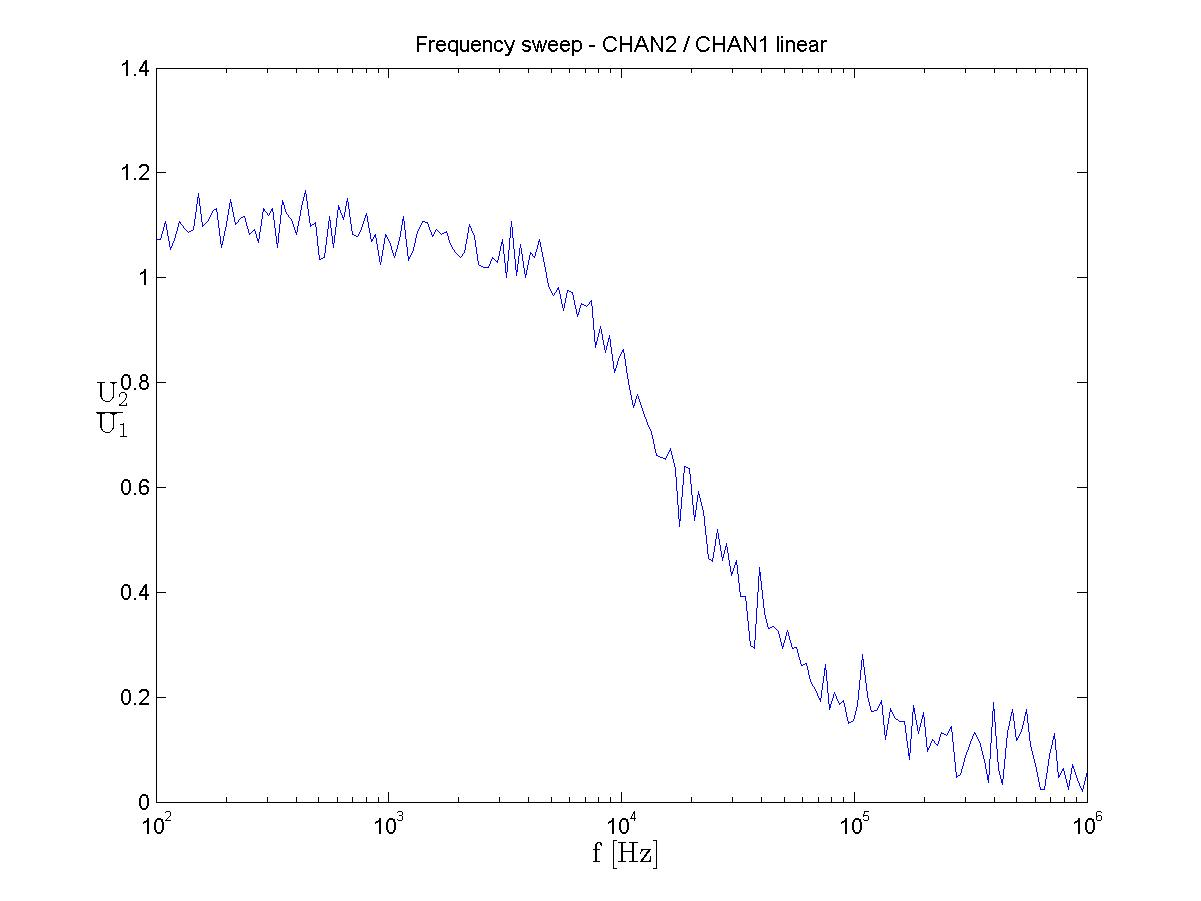
\includegraphics[width=0.8\textwidth]{versuch4/versuch4_sweep2_frequencysweep_ylinxlog.jpg}
    \caption{Frequenzgang des Integrators, veränderte Bauteilwerte}
    \label{fig:versuch4-sweep2}
\end{figure}

Der Integrator kann also auch als aktiver Tiefpassfilter eingesetzt werden, der besonders bei geringen Frequenzen ein gutes Übertragungsverhältnis von nahe $1$ zeigt.
Gegenüber dem einfachen Tiefpassfilter verliert dieser Tiefpassfilter aufgrund des Operationsverstärkers keine Leistung bei der Übertragung.



\end{document}